\section*{adi}

For each computation, there is data dependency among only one dimension, so we can compute parallelly among the other two dimensions.

We will partition the whole 3-dimensional array in 3 dimensions, as shown in Fig.\ref*{fig:adi}, so each of the subblock will have a 3-dimensional id $(i,j,k)$. Assume the size of the whole array is $N \times N \times N$, and there are $p$ processors, where $p$ is a square number. The size of a subblock is $\frac{N^3}{\sqrt p}$ and each processor will be assigned with $\sqrt p$ subblocks.

\begin{figure}[h!]
    \centering
    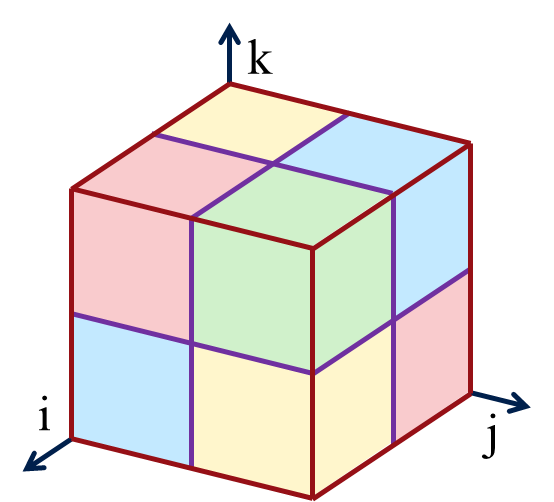
\includegraphics[width=0.3\textwidth]{fig-adi.png}
    \caption{Partition of the 3-dimensional array}
    \label{fig:adi}
\end{figure}

Since we hope that all processors can run simultaneously at the same time, for a slice in any dimension, the $\frac{N^2}{p}$ sub-blocks it contains need to be allocated to $p$ processes respectively. This requires that the subblock ids to which each processor is assigned cannot have the same i or j or k.

So here we come up with a solution to assign the subblocks to processors. We will assign the subblock $(i,j,k)$ to processor $p_{(i,j,k)}$ where $p_{(i,j,k)} = [(k-i) \mod \sqrt p] \times \sqrt p + [(j - i) \mod \sqrt p]$. To intituitively understand this, for a single processor, everytime $i$ dimension increased by 1, it will also increase the position on the $j$ and $k$ dimension by 1, so we can ensure that the subblocks with the same position in any dimension will not be assigned to the same processor.

Now suppose we are processing among the $i$ dimension and a processor reaches the boundary of the subblock in the $i$ dimension. Assume the processor is currently at subblock $(i,j,k)$, it will then calculate the owner $p_{(i+1,j,k)}$ of the next subblock $(i+1,j,k)$. Then it will send the data of the boundary of the subblock $(i,j,k)$ to the processor $p_{(i+1,j,k)}$, and receive the data of the boundary of the subblock $\left(i-1,(j-1)\mod\sqrt p,(k-1)\mod\sqrt p\right)$.

Since MPI communication can only send contiguous data, we need to pack the data before sending and unpack the data after receiving. The following is the code for packing and unpacking the data.

\begin{lstlisting}[language=C]
void pack_array(double *buffer, int i0, int j0, int k0, int i1, int j1, int k1){
    int index = 0;
    for (int k = k0; k <= k1; k++){
        for (int j = j0; j <= j1; j++){
            for (int i = i0; i <= i1; i++){
                buffer[index++] = A[k][j][i];
            }
        }
    }
}

void unpack_array(double *buffer, int i0, int j0, int k0, int i1, int j1, int k1){
    int index = 0;
    for (int k = k0; k <= k1; k++){
        for (int j = j0; j <= j1; j++){
            for (int i = i0; i <= i1; i++){
                A[k][j][i] = buffer[index++];
            }
        }
    }
}
\end{lstlisting}

The code of computing among the $i$ dimension is shown below.

\begin{lstlisting}[language=C]
for(block_i = 0; block_i < DIM_SIZE; block_i++){
    block_j = block_k = -1;
    block_id(id,&block_i,&block_j,&block_k);
    if (block_i != 0) {
        int source = block_owner(block_i - 1,block_j,block_k);
        MPI_Recv(recv_buffer,BLOCK_SIZE * BLOCK_SIZE,MPI_DOUBLE,source,0,MPI_COMM_WORLD,MPI_STATUS_IGNORE);
        unpack_array(recv_buffer,BLOCK_LOW(block_i) - 1,BLOCK_LOW(block_j),BLOCK_LOW(block_k),BLOCK_LOW(block_i) - 1,BLOCK_HIGH(block_j),BLOCK_HIGH(block_k));
    }
    for (int i = BLOCK_LOW(block_i); i <= BLOCK_HIGH(block_i); i++)
    {
        if (i == 0) continue;
        for (int j = BLOCK_LOW(block_j); j <= BLOCK_HIGH(block_j); j++)
        {
            for (int k = BLOCK_LOW(block_k); k <= BLOCK_HIGH(block_k); k++)
            {
                A[k][j][i] = A[k][j][i] * 0.4 - A[k][j][i-1] * 0.6;
            }
        }
    }
    if (block_i != DIM_SIZE - 1) {
        MPI_Barrier(MPI_COMM_WORLD);
        pack_array(send_buffer,BLOCK_HIGH(block_i),BLOCK_LOW(block_j),BLOCK_LOW(block_k),BLOCK_HIGH(block_i),BLOCK_HIGH(block_j),BLOCK_HIGH(block_k));
        int dest = block_owner(block_i + 1,block_j,block_k);
        MPI_Isend(send_buffer,BLOCK_SIZE * BLOCK_SIZE,MPI_DOUBLE,dest,0,MPI_COMM_WORLD,&request);
    }
}
MPI_Barrier(MPI_COMM_WORLD);
\end{lstlisting}

At the beginning of the loop except for the first loop, the processor will receive the data of the boundary of the subblock $(i-1,j,k)$, and then compute the data of the subblock $(i,j,k)$. After the computation, the processor will pack the data of the boundary of the subblock $(i,j,k)$ and send it to the processor $p_{(i+1,j,k)}$.

To avoid the deadlock, we use \texttt{MPI\_Isend} instead of \texttt{MPI\_Send} to send the data. The \texttt{MPI\_Isend} will not block the processor, so the processor can continue to the next loop without waiting for the data to be received by the destination processor. The \texttt{MPI\_Barrier} is used to ensure that all processors have finished the computation of the current subblock.

The code of computing among the $j$ and $k$ dimension is similar to the code above, so we will not show it here.

Finally, all data will be gathered to the processor 0, and the result will be printed out.

\begin{lstlisting}[language=C]
if(id == 0){
    double *buffer = (double *)malloc(sizeof(double) * BLOCK_SIZE * BLOCK_SIZE * BLOCK_SIZE);
    for (int source = 1; source < p; source++)
    {
        for(block_i = 0; block_i < DIM_SIZE; block_i++){
            block_j = block_k = -1;
            block_id(source,&block_i,&block_j,&block_k);
            MPI_Recv(buffer,BLOCK_SIZE * BLOCK_SIZE * BLOCK_SIZE,MPI_DOUBLE,source,0,MPI_COMM_WORLD,MPI_STATUS_IGNORE);
            unpack_array(buffer,BLOCK_LOW(block_i),BLOCK_LOW(block_j),BLOCK_LOW(block_k),BLOCK_HIGH(block_i),BLOCK_HIGH(block_j),BLOCK_HIGH(block_k));
        }
    }
    free(buffer);
} else{
    double *buffer = (double *)malloc(sizeof(double) * BLOCK_SIZE * BLOCK_SIZE * BLOCK_SIZE);
    for (block_i = 0; block_i < DIM_SIZE; block_i++)
    {
        block_j = block_k = -1;
        block_id(id, &block_i, &block_j, &block_k);
        pack_array(buffer,BLOCK_LOW(block_i),BLOCK_LOW(block_j),BLOCK_LOW(block_k),BLOCK_HIGH(block_i),BLOCK_HIGH(block_j),BLOCK_HIGH(block_k));
        MPI_Send(buffer,BLOCK_SIZE * BLOCK_SIZE * BLOCK_SIZE,MPI_DOUBLE,0,0,MPI_COMM_WORLD);
    }
    free(buffer);
}
\end{lstlisting}

If we ignore the final gathering, there are $3\sqrt p - 3$ transmits in total, and each transmit will send a boundary of size $N^2$, so the total communication cost is $O(N^2\sqrt p)$ and $O(\frac{N^2}{\sqrt p})$ for each processor.

The snapshot of the result is shown below. Since the result is too large, we use sha256 to verify the correctness of the result. It can be figured out that our parallel implementation gives the same result as the original serial implementation.

\begin{figure}[h]
    \centering
    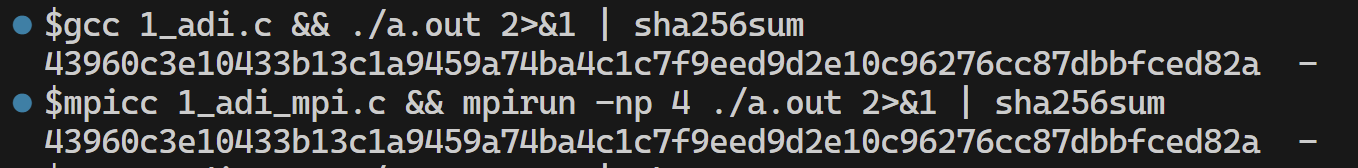
\includegraphics[width=0.8\textwidth]{fig-adi-64.png}
    \caption{Snapshot of the result ($N=64$)}
    \label{fig:adi-64}
\end{figure}

\begin{figure}[h]
    \centering
    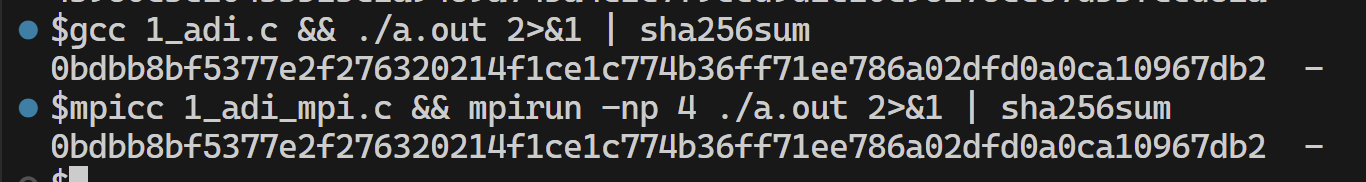
\includegraphics[width=0.8\textwidth]{fig-adi-1024.png}
    \caption{Snapshot of the result ($N=1024$)}
    \label{fig:adi-1024}
\end{figure}

\section*{floyd}

The Floyd algorithm is a classic algorithm to solve the all-pairs shortest path problem. For each loop $k$, the algorithm will update the shortest path between $i$ and $j$ by checking whether the path from $i$ to $j$ through $k$ is shorter than the current shortest path:
$$
a_{ij} = \min(a_{ij},a_{ik}+a_{kj}).
$$

We will use rowwise block striped partitioning to partition the matrix, as shown in Fig.\ref*{fig:floyd}, so each processor will be assigned with $\frac{N}{p}$ rows. Each processor will need to access the whole $k$-th row and part of the $k$-th column of the matrix. Since the part of the $k$-th column is already stored in each processor's local memory, we only need to broadcast the $k$-th row to other processors.

\begin{figure}[h!]
    \centering
    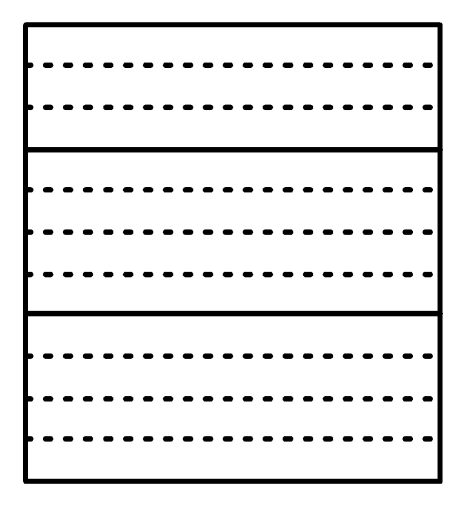
\includegraphics[width=0.15\textwidth]{fig-floyd.png}
    \caption{Partition of the matrix}
    \label{fig:floyd}
\end{figure}

The code of the Floyd algorithm is shown below.

\begin{lstlisting}[language=C]
for(int k = 0; k < N; k++) {
    MPI_Bcast(A[k], N, MPI_DOUBLE, BLOCK_OWNER(k, p, N), MPI_COMM_WORLD);
    for(int i = BLOCK_LOW(id, p, N); i <= BLOCK_HIGH(id, p, N); i++) {
        for(int j = 0; j < N; j++) {
            A[i][j] = min(A[i][j], A[i][k] + A[k][j]);
        }
    }
}
\end{lstlisting}

At the beginning of each loop, the processor responsible for the $k$-th row will broadcast the $k$-th row to other processors. Then each processor will update the shortest path between $i$ and $j$ by checking whether the path from $i$ to $j$ through $k$ is shorter than the current shortest path.

Finally, all data will be gathered to the processor 0, and the result will be printed out.

The snapshot of the result is shown below. Since the result is too large, we use sha256 to verify the correctness of the result. It can be figured out that our parallel implementation gives the same result as the original serial implementation.

\begin{figure}[h]
    \centering
    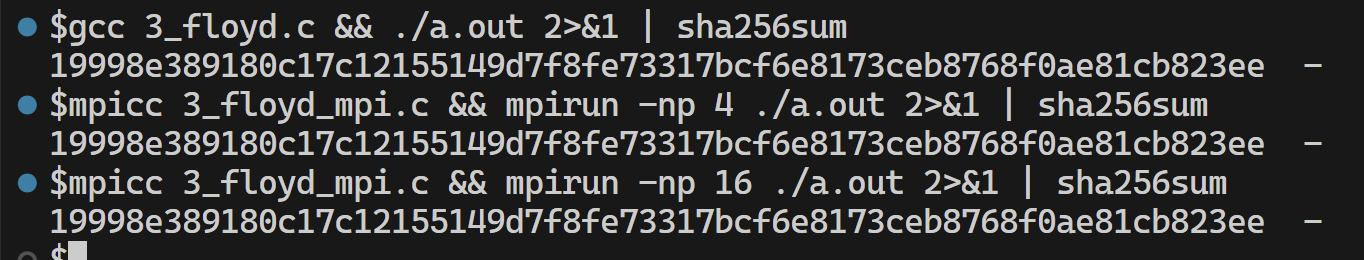
\includegraphics[width=0.8\textwidth]{fig-floyd-1024.png}
    \caption{Snapshot of the result ($N=1024$)}
    \label{fig:floyd-1024}
\end{figure}